\section{Analysis}

\begin{table}[htb!]
% \vspace{-9pt}
\setlength{\tabcolsep}{6pt}
\centering
  \caption{Ablation study in the retinal fundus segmentation. Details of the experiment can be found in Sec~\ref{sec:abl_ue}.}
  \vspace{-0.3cm}
  \begin{adjustbox}{width=0.999\linewidth}
    \begin{tabular}{c|ccccc|c}
\hlineB{3}
\multirow{2}{*}{Methods}     & Site A & Site B & Site C & Site D & Site E & Average \\ \cline{2-7}
& \multicolumn{6}{c}{\textbf{Dice Score Metric $\uparrow$ (DSC, mean$\pm$std )}} \\ \hline \hline

\textit{No Adapt} & 65.60\small{$\pm$5.78} & 74.65\small{$\pm$4.88} & 63.15\small{$\pm$7.30} & 68.11\small{$\pm$5.49} & 75.34\small{$\pm$1.01} & 69.37\\ \hline

\textit{w/o $\mathcal{U}$}      &  77.09\small{$\pm$1.90}      & 83.24\small{$\pm$2.01}       &  80.50\small{$\pm$1.44}      &  78.32\small{$\pm$1.55}      &    83.18\small{$\pm$2.18}    &  80.47       \\
\textit{w/o priors} &   79.51\small{$\pm$0.80}     & 79.36\small{$\pm$1.13}       &  77.40\small{$\pm$1.89}      &    77.29\small{$\pm$1.77}    &  80.00\small{$\pm$1.93}      &    78.71     \\
\hline
Ours &  82.53\small{$\pm$1.52} &  88.98\small{$\pm$0.89}      &  88.73\small{$\pm$0.70}      &  90.25\small{$\pm$1.33}      &   91.83\small{$\pm$0.71}     &   \textbf{88.46}    \\
\hlineB{3}
\end{tabular}
  \end{adjustbox}
  \label{tab:tabel_abl1}
\end{table}

% To assess the effectiveness of the universe embeddings, multi-graph matching, and the entire test-time paradigm, we conducted a series of ablation experiments on the retinal fundus datasets. The experimental settings remained consistent with those in Sec.~\ref{exp_setup}. For more detailed analysis, please refer to the supplementary material.

\subsection{Effectiveness of the Universe Embeddings}
\label{sec:abl_ue}
The universe embeddings $\mathcal{U}$ play a crucial role in incorporating morphological priors from medical images, resulting in an assignment matrix that projects each node to the \textit{universe of nodes}. To validate the effectiveness during the TTA, we conducted the following experiments: (1) Without universe embeddings (denoted as \textit{w/o $\mathcal{U}$}), the universe matching assignment matrix $\bold{U}$ is initialized following the setting in \cite{wang2020graduated} (i.e. $\bold{U}=1/d+10^{-3}z$, where $z\sim N(0,1)$), leading to random matching between the nodes and the universe; (2) Without morphological priors but with $\mathcal{U}$ (denoted as \textit{w/o priors}). As shown in Table~\ref{tab:tabel_abl1}, the performance in (1) is slightly better than in (2) by 1.76\% in terms of DSC on average. However, when using the pre-trained $\mathcal{U}$ derived from the source model, the segmentation results show a significant improvement. This highlights the effectiveness of the pre-trained morphological priors embedded in $\mathcal{U}$ for medical imaging tasks.

\begin{figure}[!t]
    \centering
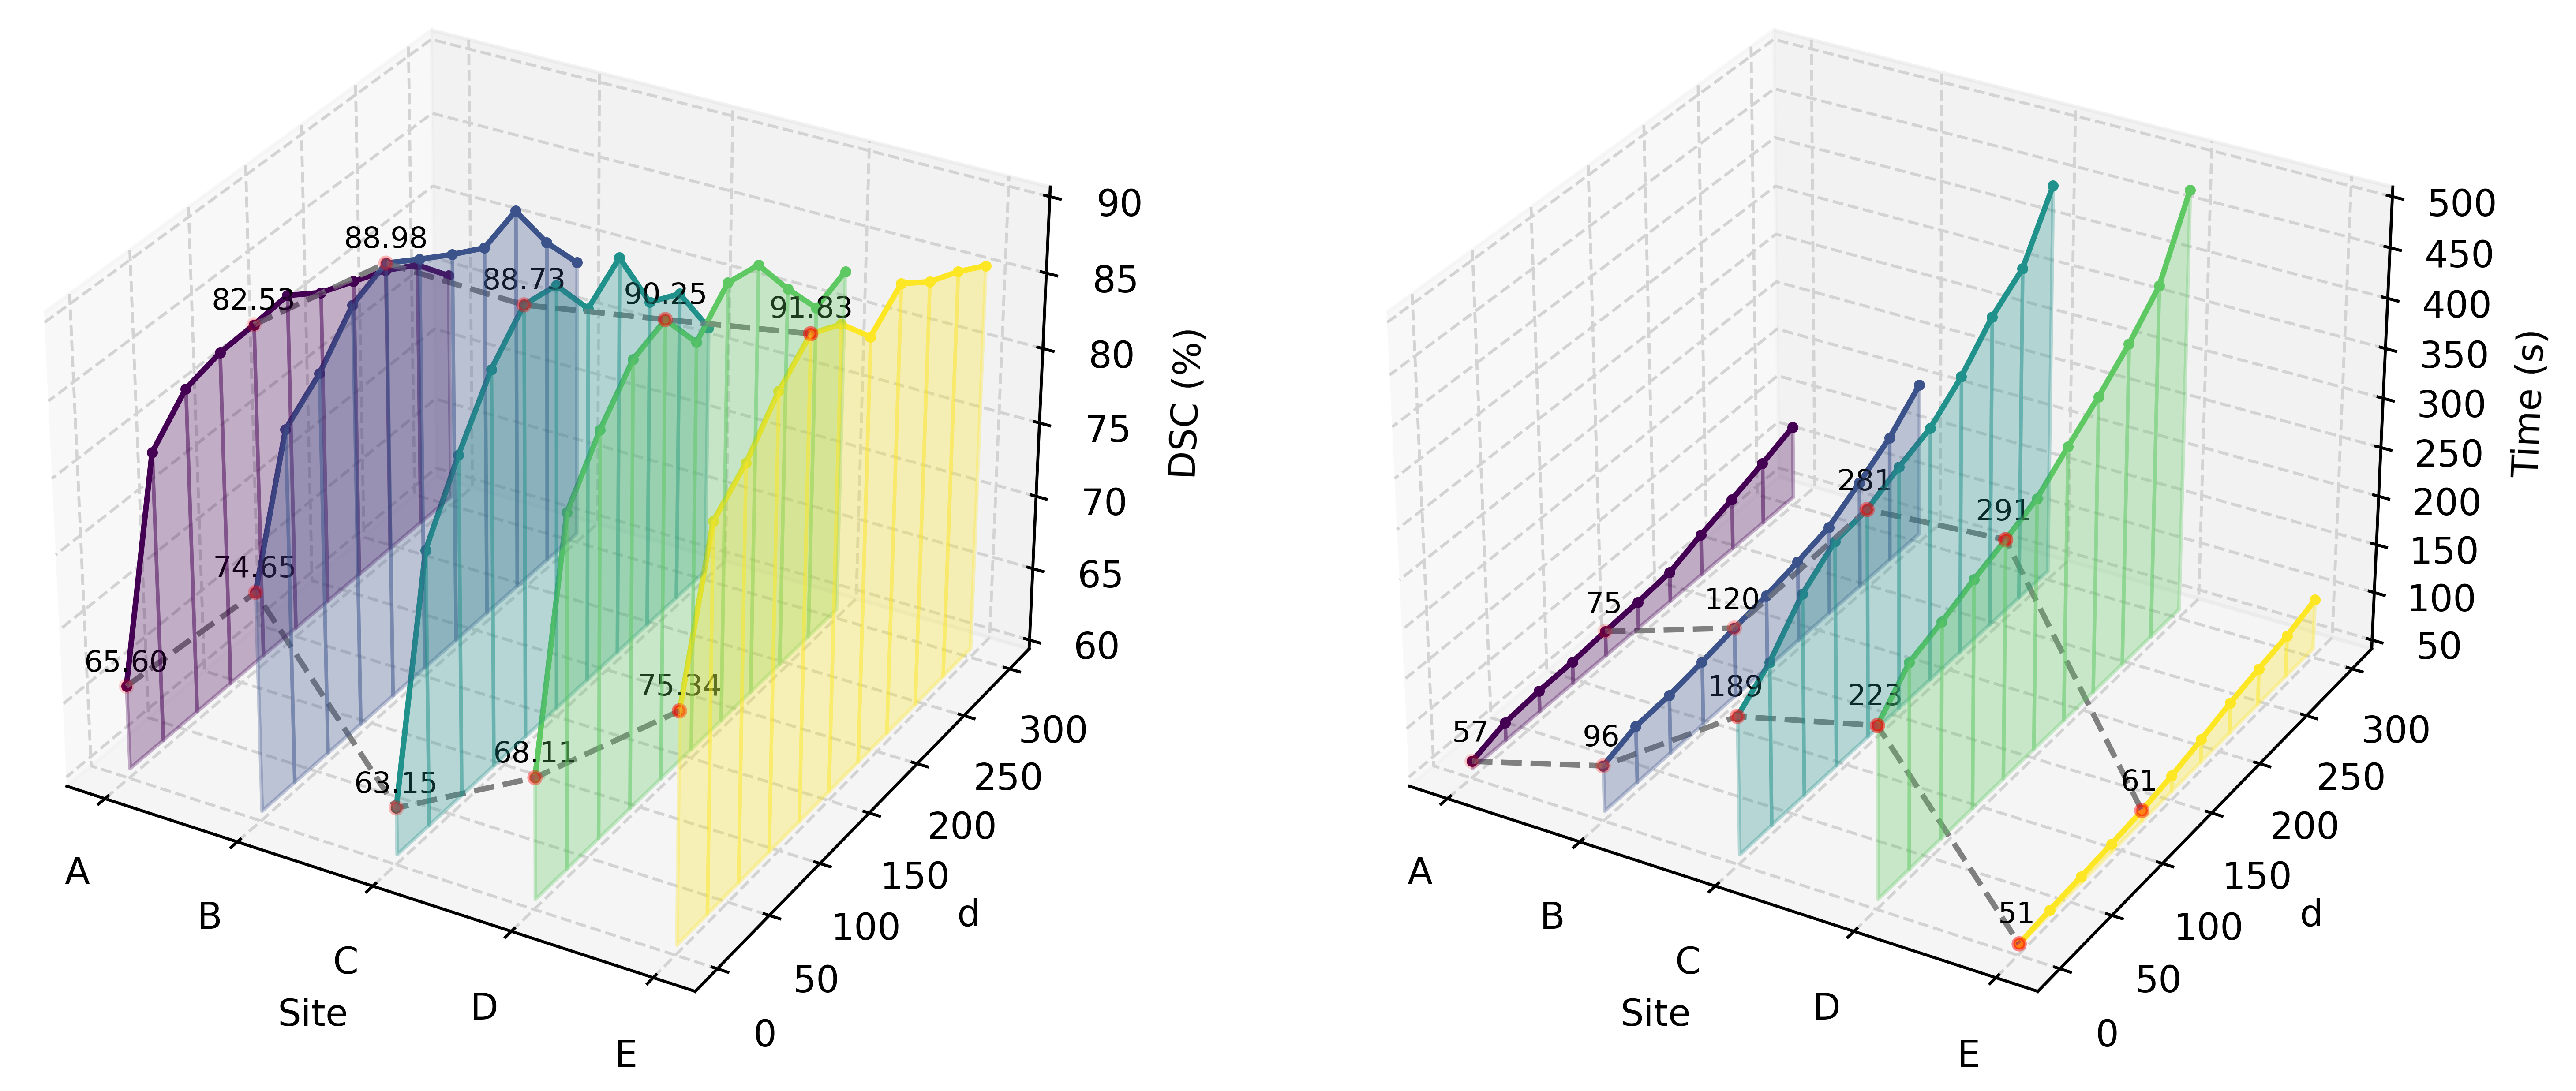
\includegraphics[width=0.999\linewidth]{Figures/comparison_dsc_time_labeled.png}
    % \vspace{-10pt}
    \caption{The performance of DSC (\%) and inference time (s) with different universe sizes $d$ are shown, with the experimental setup identical to that in Table~\ref{tab:tabel_fundus}. The first curve represents the \textit{No Adapt} baseline ($d = 0$), while the subsequent curve corresponds to the results obtained with a universe size of $ d = 120$.}
     \vspace{-0.5cm}
    \label{fig:universe_d}
\end{figure}

\vspace{-5pt}
\subsection{Effectiveness of the Universe Size}
The universe size $d$ directly impacts both the matching accuracy and computational efficiency, and its selection depends on the number of sampled nodes. Previous works~\cite{bernard2019hippi,wang2020graduated,nurlanov2023universe}, ensured that the $d$ matched the number of nodes in each graph by labeling an equal number of keypoints. In our experiments, $d$ is determined by the spatially-uniform sampling described in Sec~\ref{sec:graph_generation}, and we empirically set $d = 100\times (n+1) s^{-1}$, where $s$ is the sampling step and $n$ is the number of segmentation categories required for the task. We evaluated several $d$, with the results shown in Fig.~\ref{fig:universe_d}. We observe that excessively small or large step sizes—resulting in too many or too few sampled nodes—negatively impact both training speed and performance. However, when $d$ is within a reasonable range (in this experiment, $s \in[2, 10]$ i.e. $d \in [30, 150]$.), the model maintains good scalability and performance.

\begin{table}[htb!]
\vspace{-9pt}
\setlength{\tabcolsep}{8pt}
\centering
  \caption{Comparison of common variables and performance between pairwise matching and multi-matching, using the same experimental setup as in Table~\ref{tab:tabel_fundus}. Both methods follow the graph construction in Sec.~\ref{sec:graph_generation}.}
  \vspace{-0.3cm}
  \begin{adjustbox}{width=0.979\linewidth}
    \begin{tabular}{r|cc|l}
\hlineB{3}
\multirow{2}{*}{param} & \multicolumn{2}{c|}{Site A-E Average}              & \multirow{2}{*}{description}      \\ \cline{2-3}
&Pairwise~\cite{wang2019learning}         & Multi-Matching (Ours) & \\ \hline \hline
lr                     & $10^{-3}$ & $10^{-3}$ & learning rate \\
batch & 4 & 4  & batch size in  inference  \\
$h$ & 256 & 256  & dimension of node feature\\
$\tau$  & 0.05   & 0.05  & regularization factor of Sinkhorn \\
\textit{Iter} & 20 & 20 & max iterations of Sinkhorn        \\
$d$    & -  & 120 & universe size \\ \hline
DSC $\uparrow$  &  84.63   &  \textbf{88.46}  & dice score metric (\%) \\
time $\downarrow$& 0.930 &  \textbf{0.392}   & inference time per image (s/img)  \\
Param $\downarrow$ & 1.071 & \textbf{0.658} & parameter count (M) \\
FLOPs $\downarrow$&  15.35  &  \textbf{4.255}  &   floating point operations per second (G)  \\ \hlineB{3}
\end{tabular}

  \end{adjustbox}
  \label{tab:tabel_abl_matching}
\end{table}
\vspace{-0.5cm}
\subsection{Multi-Matching vs. Pairwise Matching}
Compared to pairwise matching, multi-matching uses cycle-consistency for global optimization, which helps avoid local optima in pairwise. Moreover, joint optimization reduces the computational complexity of large-scale matching. By incorporating morphological consistency constraints, multi-matching exhibits greater robustness. To validate these claims, we conducted experiments comparing the two approaches. 
For the pairwise matching method, we adopted the benchmark approach~\cite{wang2019learning} and applied the same graph construction process as in multi-matching. The comparison results are presented in Table~\ref{tab:tabel_abl_matching}. It is evident that multi-matching outperforms pairwise matching in terms of DSC, inference time, parameters and FLOPs.
The inference time of multi-matching was reduced by approximately 57.85\% compared to pairwise matching, while segmentation accuracy improved by 3.83\% in DSC.